This chapter deals with the Android operating system and its architecture. Android platform is quite different from
Java platform. They use the same language for source code of applications and the build process is also similar but the
differences cause that they are not fully compatible.

In Section~\ref{AndroidIntroductionSection}, Android and its history is presented. Architecture of this platform is
described in Section~\ref{AndroidArchitectureSection} and part of this architecture -- Android runtime -- is discussed
in more detail in Section~\ref{AndroidRuntimeSection}. Basic components of Android application are presented in
Section~\ref{AppStructureSection} and the build process of Android source code and the development environment is
described in Section~\ref{BuildProcessSection}.

\section{Introduction}\label{AndroidIntroductionSection}
Android~\cite{AndroidBook, AndroidProgBook} is a~mobile operating system developed by Google. It is an~open-source
system based on the Linux kernel mainly used in mobile devices such as smartphones, tablets and smart watches but it can
also be found in devices such as set-top boxes, media players and other electronics.

Android Inc. was founded in California USA in 2003. Google Inc. bought Android two years later. In 2007, Google acquired
several patents in the field of mobile devices and at the same year on November 5, there was an~official presentation
of companies association (Open Handset Alliance) which aims to create open standards for mobile devices. The first
smartphone with Android released on October 22, 2008.

Table~\ref{AndroidHistoryTable} presents a~brief history of the Android operating system. It describes release dates of
major versions, version numbers, code names, API levels and distributions in the last column. As can be seen from
version 1.5, every major version has its own codename represented by a~popular food. API level indicates that version
brings changes in its programming interface and the most important column shows the distrubiton of each version.
According to this, it may be decided for which versions still makes sense to develop an~application.

\begin {table}[h!]
    \catcode`\-=12
    \begin{tabular}{|l|c|l|c|c|}
        \hline
        \textbf{Release date} &
        \textbf{Version} &
        \textbf{Codename} &
        \textbf{API level} &
        \multicolumn{1}{p{2.3cm}|}{\centering \textbf{Distribution} [\%]} \\ \hline \hline
        September 23, 2008 & 1.0 -- 1.1   & --                 & 1 -- 2   & \multirow{4}{*}{\textless~0.1}
        \\ \cline{1-4}
        April 27, 2009     & 1.5          & Cupcake            & 3        &                     \\ \cline{1-4}
        September 15, 2009 & 1.6          & Donut              & 4        &                     \\ \cline{1-4}
        October 26, 2009   & 2.0 -- 2.1   & Eclair             & 5 -- 7   &                     \\ \hline
        May 20, 2010       & 2.2 -- 2.2.3 & Froyo              & 8        & 0.3                 \\ \hline
        December 6, 2010   & 2.3 -- 2.3.7 & Gingerbread        & 9 -- 10  & 5.7                 \\ \hline
        February 22, 2011  & 3.0 -- 3.2   & Honeycomb          & 11 -- 13 & \textless~0.1       \\ \hline
        October 18, 2011   & 4.0 -- 4.0.4 & Ice Cream Sandwich & 14 -- 15 & 5.3                 \\ \hline
        July 9, 2012       & 4.1 -- 4.3   & Jelly Bean         & 16 -- 18 & 39.2                \\ \hline
        October 31, 2013   & 4.4 -- 4.4.4 & KitKat             & 19 -- 20 & 39.8                \\ \hline
        November 12, 2014  & 5.0 -- 5.1.1 & Lollipop           & 21 -- 22 & 9.7                 \\ \hline
    \end{tabular}
    \centering
    \caption{Android version history~\cite{Dashboards}.}
    \label{AndroidHistoryTable}
\end{table}

\section{Architecture}\label{AndroidArchitectureSection}
This section deals with the architecture of Android system~\cite{AndroidDevBook} which consists of six layers.
Figure~\ref{AndroidArchitectureFigure} and following paragraphs describe this architecture starting with the kernel
layer and ending with the applications.

\paragraph{Linux kernel}
The lowest layer stands between hardware device and other architecture layers. Android is based on a~special version of
Linux kernel and several accessories such as memory management system, the Binder IPC driver and others. Since the
beginning, Android was built on the Linux 2.6 kernel. The latest version 5 from Table~\ref{AndroidHistoryTable} runs on
the kernel 3.4.

\paragraph{Hardware abstraction layer}
Hardware abstraction layer (HAL) is standard interface which allows to Android system calls drivers layer while it does
not have to care what is the implementation of drivers and hardware in lower layers. For each piece of hardware should
be a~driver and matching HAL providing hardware options.

\paragraph{Libraries}
Above the HAL is a~layer of native libraries. These libraries are written in C~or C++ language and they can be accessed
through the Android Standard Development Kit (SDK) but if direct access is required, it is possible to do that through
the Native Development Kit (NDK). The layer includes the following libraries:

\begin{itemize}
    \item \textbf{Surface manager} -- library for composing different drawing surface windows on the screen.
    \item \textbf{Media Framework} -- provides various multimedia codecs for playing and recording video in various
    formats.
    \item \textbf{SQLite} -- a~database engine for the use in data storage.
    \item \textbf{WebKit} -- a~browser engine for displaying web content.
    \item \textbf{Libc} -- the standard library of the C programming language.
    \item \textbf{OpenGL ES} -- a~library for support 2D and 3D graphics and hardware accelerated rendering.
    \item \textbf{Audio Manager} -- a~library for working with audio of device.
    \item \textbf{FreeType} -- a~library for bitmap and vector font rendering.
    \item \textbf{SSL} -- a~library for the use of encryption protocol for secure internet communications.
\end{itemize}

\paragraph{Android runtime}
Android runtime layer is located next to the native libraries. This layer consist of two parts. The first one is the
Core Libraries and the second one is the Dalvik Virtual Machine. The Core libraries can be further subdivided into two
parts: Java libraries and Android libraries. Section~\ref{AndroidRuntimeSection} describes the details of this layer.
\\
\begin{figure}[h!]
    \centering
    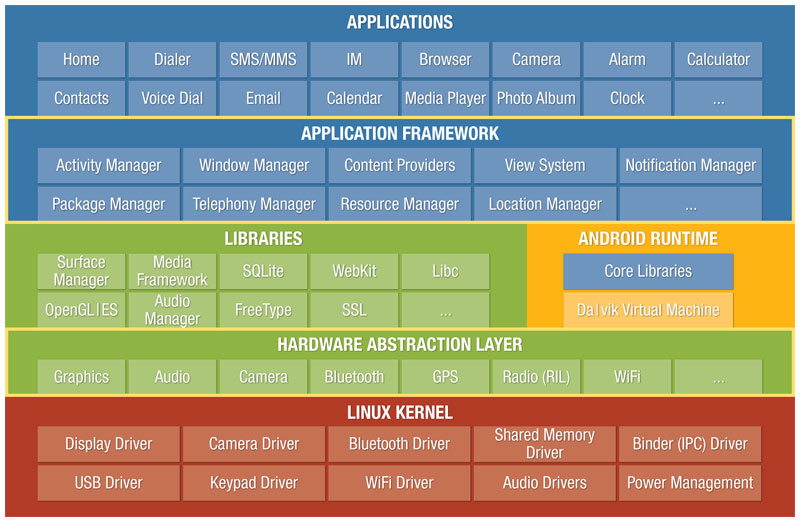
\includegraphics[scale=0.54]{fig/android_architecture.jpg}
    \caption{Android architecture~\cite{AndroidArch}.}
    \label{AndroidArchitectureFigure}
\end{figure}

\paragraph{Application framework}
Application framework layer provides many high-level services to applications in the form of Java libraries. For
developers, this is the most important layer that allows access to the device services. The Application framework
includes the following parts:
 
\begin{itemize}
    \item \textbf{Activity manager} -- controls all aspects of running activities. It manages all Services and
    Activities described in Section~\ref{AppStructureSection}.
    \item \textbf{Windows manager} -- provides services for windows management such as visibility and arrangement. It
    also takes care about animation on the screen.
    \item \textbf{Content Providers} -- allows to work with a~content of other applications, it encapsulates the data
    and provides mechanisms for defining data security.
    \item \textbf{View System} -- a~set of basic blocks that is used to build the application user interface. The basis
    of every graphical component is the \texttt{View} class which is represented by a~rectangular area on the screen.
    \item \textbf{Notification manager} -- provides the possibility to inform the user about some action that happened
    in the background. Notifications can take different forms like LED flashing, vibrating, ringing or notification on
    the screen.
    \item \textbf{Package manager} -- allows obtaining of various information about applications that are currently
    installed on device.
    \item \textbf{Telephony manager} -- provides access to telephone services of device. These services include SIM
    card, network, cellphone or other information.
    \item \textbf{Resource manager} -- allows access to non-code resources such as color settings, layouts and strings.
    Separating of resources from code helps to better manage the various characteristic without modifying the code.
    \item \textbf{Location manager} -- provides access to the location services. These services allow periodical
    receiving of geographic coordinates and therefore it is possible to track device current location.
\end{itemize}

\paragraph{Applications}
The last and highest layer consists of the applications themselves. These comprise both pre-installed applications and
applications that have been added over time from the Android store or another way.

\section{Android runtime}\label{AndroidRuntimeSection}
Both Android runtime and Java Runtime Edition include a~virtual machine and Java SE API. In case of Android,
its runtime contains special virtual machine named Dalvik Virtual Machine (DVM) and API lacks several Java packages and
classes and contains special Android libraries.

\subsubsection{Dalvik Virtual Machine}
DVM is a~virtual machine that is developed since 2005 and it is included into the system due to the fact that JVM was
not licensed as open-source in the past. The second reason is the optimization for mobile devices.

Each application runs on an~Android device within its own instance of DVM (i.e. not as a~process in the Linux kernel).

Running applications on a~virtual machine has many advantages. First, it operates in a~sandbox and thus can not
interfere with the operating system or other applications. Secondly, it makes the application platform independent and
therefore can be run on any hardware. Advantages also include memory usage which makes the DVM better adaptable for use
on mobile devices.

An~application code must be always transformed from a~standard \texttt{.java} file into bytecode but it is different in
Java applications after this point. Bytecode is not executed by DVM but instead of that it is converted by Dex tool to
Dalvik executables (\texttt{.dex} format). The whole process is described in Section~\ref{BuildProcessSection}.


\paragraph{Java libraries}
Most of Android applications are written using Java. Android contains libraries based on Apache Harmony Project that is
an~open-source Java implementation. These libraries are a~subset of the Java SE platform. They do not contain all of the
packages. For example, \texttt{java.awt} or \texttt{java.swing} libraries are replaced by Android user interface classes
and packages. More detailed comparison can be found in Chapter~\ref{PortingChapter}.

\paragraph{Android libraries}
Android libraries contain specific packages that provide all the functionality of Android devices. Libraries are written
in Java and they include the following packages:

\begin{itemize}
    \item \texttt{android.app} -- provides access to the application model and it is the base of all applications.
    \item \texttt{android.content} -- classes for accessing and publishing data applications.
    \item \texttt{android.database} -- classes for data access and database manipulation.
    \item \texttt{android.graphics} -- library for screen low-level 2D graphics drawing.
    \item \texttt{android.hardware} -- provide access to hardware features such as cameras and sensors.
    \item \texttt{android.media} -- library for handling with multimedia.
    \item \texttt{android.text} -- library for manipulation and rendering of strings.
    \item \texttt{android.util} -- common tools such as data manipulation and time utilities, conversions between
    numbers and strings and other classes.
    \item \texttt{android.view} -- basic library for building a~graphical user interface.
    \item \texttt{android.webkit} -- libraries for working with web content.
\end{itemize}

\section{Application structure}\label{AppStructureSection}
In this section, anatomy of application is described. Application consist of the various components and blocks whose
description follows.

\paragraph{Activities}
Activities represent one single screen of user interface. Typically after an~application start, the main activity is
displayed and from there, another activity can be started or other operations can be performed. When a~new activity is
started, the previous one is stored in a~Last In First Out stack. After pressing the back button, the stored Activity is
invoked again.

\paragraph{Fragments}
Fragment is a~modular section of an~activity which has its own lifecycle. They represent a~portion of Activity, one
Activity can contain more fragments and they are used for adapting the layout of components on various screens.

\paragraph{Services}
Services are components that run in the background performing long-term tasks. They do not provide a~user interface.
Services may be still active in the background while other applications is running. For example, a~service might be
playing music or downloading from the Internet.

\paragraph{Content providers}
Content providers store and load data to make them available for other applications. Through the content providers,
other applications may modify or manipulate specific data. An~example might be a~content provider that manages the
contact information on the device.

\paragraph{Intents}
Intents are messages between one component and other component. Intent can be sent to inside or outside of
an~application and it means that one application can communicate with another. Three types of application components
are supported for Intents communication -- Activities, Services, and Broadcast receivers -- and there are two types of
intents -- Explicit and Implicit. Explicit intents specify the component to start by name. Implicit intents do not
specify the component, another application can handle it and makes appropriate response.

\paragraph{Broadcast receivers}
These components are used to listen message notifications (Intents) from outside (other application or system) or from
inside of the application. After receiving the message, receivers can initiate appropriate reaction. An~example might be
an~incoming Short Message Service (SMS) or low battery notification.

\paragraph{Application resources}
Android application consists not only of Java files but also of the resources that are separated from the source code.
These resources include:

\begin{itemize}
    \item \textbf{Animation resources} -- define predefined animation.
    \item \textbf{Color state list resources} -- define color change based on the \texttt{View} class state.
    \item \textbf{Drawable resources} -- define different bitmaps or XML (eXtensible Markup Language) graphics files.
    \item \textbf{Layout resources} -- define the layout of application components.
    \item \textbf{Menu resources} -- define content of application menus.
    \item \textbf{String resources} -- define string and string arrays.
    \item \textbf{Style resources} -- define the appearance and format of ui elements.
\end{itemize}

\paragraph{Application manifest file}
Each application must have an~\texttt{AndroidManifest.xml} file. This file contains information about application with
regard to Android and it has to be placed in root directory of project. It has to contain a~unique package name for the
application, the declaration of used Activity and Service components, application permissions to the protected parts of
the API (such as access to the camera, etc.). A~minimum API level, list of connected and used libraries and other
important informations about application have to also be declared. Android manifest is together with resources compiled
by \texttt{aapt} tool to \texttt{R.java} file. Thanks to this, the manifest informations are available in the source
code.

\begin{figure}[h!]
    \centering
    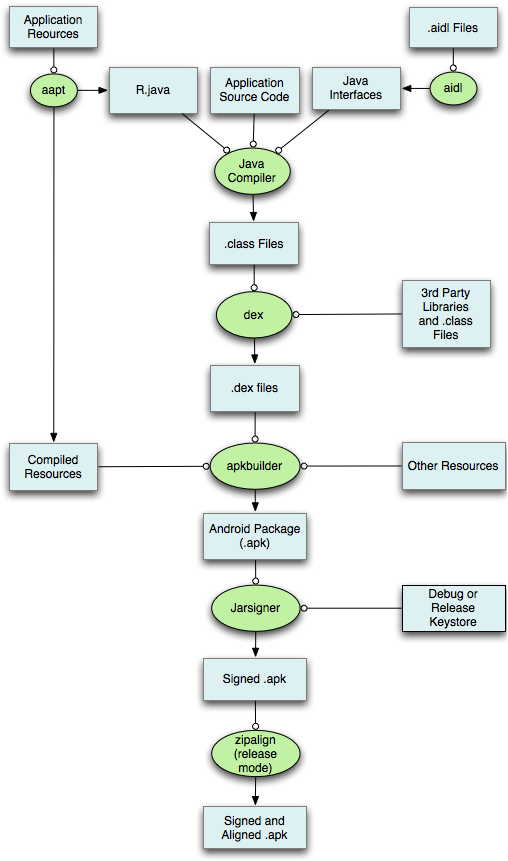
\includegraphics[scale=0.5]{fig/build.png}
    \caption{Android build process~\cite{AndroidDev}.}
    \label{BuildProcessFigure}
\end{figure}

\section{Build Process}\label{BuildProcessSection}
Build process is the way how \texttt{.apk} package is produced from Android project. APK (Android application package)
file is a~file format used for distribution and installation of application software to Android devices. It contains all
of the necessary files to run an~application. Figure~\ref{BuildProcessFigure} shows how APK package is created from
Java source code and resources including Android manifest file. The individual steps are:

\begin{enumerate}
    \item The Android Asset Packaging Tool compiles resource files and \texttt{AndroidManifest.xml} and produces
    \texttt{R.java}. Resource references from Java code are then linked to this file.
    \item \texttt{aidl} tool coverts all \texttt{.aidl} interfacese to Java interfaces. Aidl files are interfaces used
    for interprocess communication between client and service.
    \item Java compiler takes and compiles \texttt{R.java} file, application source code and Java interfaces to
    bytecode. Bytecode is stored in \texttt{.class} output files.
    \item Any third party libraries and \texttt{.class} files are converted by Dex tool to Dalvik byte code which is
    stored in \texttt{.dex} files.
    \item Other uncompiled resource (eg. images), compiled resource and \texttt{.dex} files are processed by
    \texttt{apkbuilder} tool which packs them to \texttt{.apk} file.
    \item Once the \texttt{.apk} file is created, it must be signed by debug or release key. \texttt{jarsigner} tool
    provides signing and creates signed \texttt{.apk} file.
    \item Finally, if the application is being signed in release mode, \texttt{zipalign} tool align the \texttt{.apk}
    file. It creates signed and aligned \texttt{.apk} file which is not so memory consuming.
\end{enumerate}

Following paragraphs presents environment for developing of Android applications and its build tool. These two systems
automate development and the build process which is described above.

\paragraph{Android studio}
In the past, Google has supported two developer tools for developing Android applications. From the very beginning,
Eclipse with Android plugin was primary environment. Now, the official environment for development of Android
applications is called Android studio~\cite{AndroidDev}. It is a~multiplatform application which provides tools to
facilitate application development. Android studio is based on the IntelliJ IDEA Java IDE and Gradle language is used as
default build system.

\paragraph{Gradle build system}
Gradle build system~\cite{Gradle} is a~project automation tool which is built on the concepts of Apache Ant~\cite{Ant}
and Apache Maven~\cite{Maven} tools. It is used as default build system in Android studio and using Tasks from Android
Gradle plugin automates the entire build process described above. A~Task represents a~process which launches some
sections of Gradle build code. Standard Tasks for every Android application are:

\begin{itemize}
  \item \texttt{gradle clean} -- cleans project and deletes the build directory.
  \item \texttt{gradle assemble} -- builds the project.
  \item \texttt{gradle check} -- runs checks and tests.
  \item \texttt{gradle build} -- runs both assemble and check.
  \item \texttt{gradle assembleDebug} -- creates debug \texttt{.apk} file.
\end{itemize}
